\documentclass[tikz]{standalone}
\usetikzlibrary{automata,positioning}
\begin{document}
  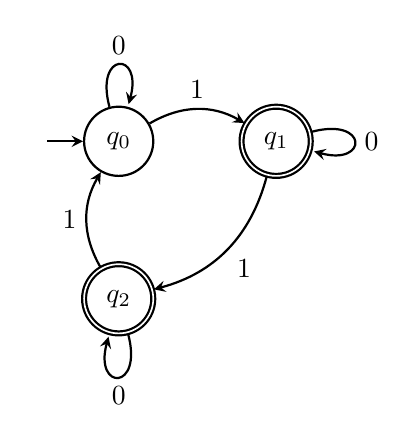
\begin{tikzpicture}[>=stealth,node distance=2cm,on grid,auto, thick, initial text=]
    \node[state,initial] (q_0) {$q_0$};
    \node[state,accepting] (q_1) [right=of q_0] {$q_1$};
    \node[state,accepting] (q_2) [below=of q_0] {$q_2$};
    
    \path[->]
    (q_0) edge [loop above] node {0} (q_0)
    (q_0) edge [bend left] node {1} (q_1)
    (q_1) edge [loop right] node {0} (q_1)
    (q_1) edge [bend left] node {1} (q_2)
    (q_2) edge [loop below] node {0} (q_2)
    (q_2) edge [bend left] node {1} (q_0);
  \end{tikzpicture}

\end{document}